\subsection{Unlocking the Perfect Terminating Resistance for Your Beverage Antenna!}

\begin{tcolorbox}[colback=gray!10, colframe=black, title=E9H06] What indicates the correct value of terminating resistance for a Beverage antenna?\\
\begin{enumerate}[label=\Alph*.]
    \item Maximum feed point DC resistance at the center of the desired frequency range
    \item Minimum low-angle front-to-back ratio at the design frequency
    \item Maximum DC current in the terminating resistor
    \item \textbf{Minimum variation in SWR over the desired frequency range}
\end{enumerate} \end{tcolorbox}

\subsubsection{Concepts Related to Beverage Antennas and Terminating Resistance}

Beverage antennas are a type of low-profile, long-wire antenna, primarily designed for receiving radio signals. They are known for their low-angle radiation pattern and are often used for long-distance communication, especially in the shortwave bands. One critical factor in optimizing the performance of a Beverage antenna is the value of the terminating resistance.

The terminating resistance plays a crucial role in ensuring that the antenna operates with an optimal standing wave ratio (SWR). The SWR is a measure of how effectively radio frequency (RF) power is transmitted from the power source, through the transmission line, and into the load (in this case, the antenna). An SWR of 1:1 signifies perfect matching, where all the power is radiated by the antenna without reflections.

In this context, the correct answer indicates that the terminating resistance should be chosen to minimize the variation in SWR across the desired frequency range (option D). A high variation in SWR can lead to inefficient transmission, signal loss, and suboptimal performance.

\subsubsection{Mathematical Analysis}

To calculate the required terminating resistance, we can use the formula for SWR:

\[
\text{SWR} = \frac{Z_L}{Z_0}
\]

where \( Z_L \) is the load impedance (the antenna system), and \( Z_0 \) is the characteristic impedance of the feed line. To achieve an SWR of 1:1, we need:

\[
Z_L = Z_0
\]

Additionally, for the Beverage antenna, the optimal terminating resistance can typically be around 600 ohms, as this value tends to minimize the SWR variation across a wide frequency range.

\subsubsection{Conclusion}

Thus, it is crucial to select the terminating resistance that minimizes SWR variation to ensure efficient operation of the Beverage antenna. This enhances the reception of signals and prevents the loss due to reflections that occur when the impedance is mismatched.

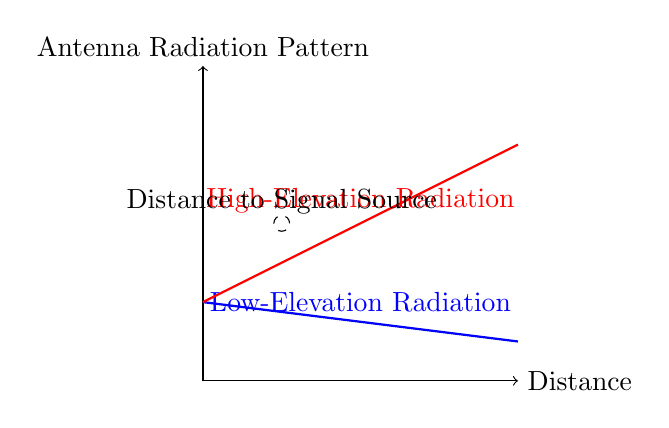
\begin{tikzpicture}
    \draw[->] (0,0) -- (0,4) node[above] {Antenna Radiation Pattern};
    \draw[->] (0,0) -- (4,0) node[right] {Distance};
    \draw[blue,thick] (0,1) -- (4,0.5) node[midway,above] {Low-Elevation Radiation};
    \draw[red,thick] (0,1) -- (4,3) node[midway,above] {High-Elevation Radiation};
    \draw[dashed] (1,2) circle(0.1) node[above] {Distance to Signal Source};
\end{tikzpicture}
